\section{Thesis Plan}
\label{sec:1_introduction_methodology}
\begin{figure}[!ht]
    \centering
    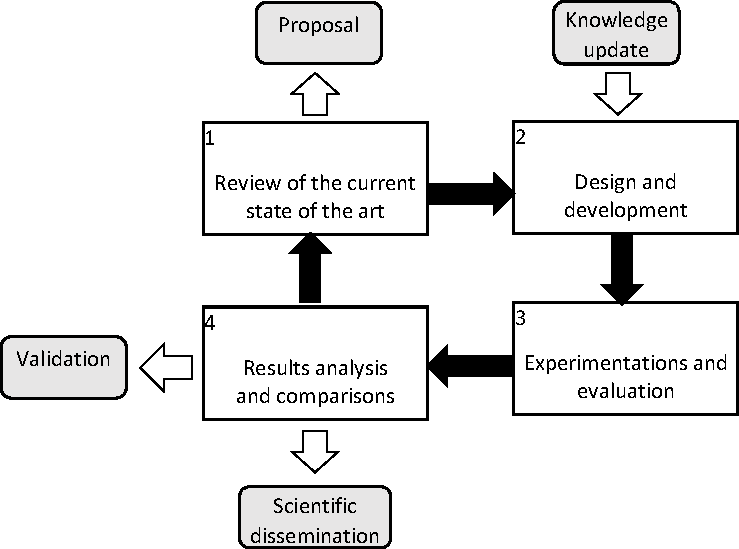
\includegraphics[width=.8\textwidth]{1_introduction/figures/fig_research-methodo.pdf}
    \caption{The Research Plan of Thesis.}
    \label{ch1:research-emthodo}
\end{figure}

The research in this thesis is progressing rapidly due to technological advancements and continuous contributions in machine learning (ML). An iterative research methodology was followed, where each cycle builds upon the knowledge gained in the previous phase, leading to increasingly effective and original solutions as shown in Fig. \ref{ch1:research-emthodo}. The phases of this research methodology are as follows:

\begin{enumerate}
    \setlength{\itemsep}{0pt}
    \setlength{\parskip}{0pt}
    \item \textbf{Review of the current state-of-the-art:} Investigate existing research to identify challenges and inform the design of a solution.
    \item \textbf{Design and development:} Design a novel solution using updated knowledge to address the identified challenges.
    \item \textbf{Experimentation and evaluation:} Test the solution through experimentation, using established criteria for comparison.
    \item \textbf{Results analysis and comparison:} Analyze and compare results with state-of-the-art to determine the effectiveness of the solution, and disseminate the findings.
\end{enumerate}

